%====================================================================
%====================================================================
\subsection{(Joint) species distribution models}
%====================================================================
\frame{\frametitle{(Joint) species distribution models} 

  \paragraph{Aim.} 
  Describe/understand the relationships that living species share with each other and with their environment (biogeography, community ecology). 

  \bigskip \bigskip \pause 
  \paragraph{Species distribution models.} 
  $n$ sites, $x_i =$ vector of environmental descriptors for site $i$, $Y_i =$ number of individual from the species of interest observed in site $i$:
  $$
  Y_i \sim \Fcal(\cdot; x_i, \emphase{\beta}).
  $$
  $\to$ Generalized linear (mixed) model \refer{ElL09,ZIW09}

  \bigskip \bigskip \pause
  \paragraph{Joint species distribution models.} 
  Same, but $Y_i = (Y_{i1}, \dots Y_{ip}) =$ vector of counts for $p$ species of interest observed in site $i$:
  $$
  Y_i \sim \Fcal_p(\cdot; x_i, \emphase{\beta}, \emphase{\Sigma})
  $$
  $\to$ Multivariate generalized linear mixed model  \refer{WBO15,OvA20}
  
}

%====================================================================
\frame{\frametitle{Poisson log-normal model}

  \bigskip
  \paragraph{A joint species distribution model:} 
  Poisson-log normal distribution \refer{AiH89,CMR21}
  \begin{align*}
    & \text{in each site $i = 1 \dots n$:} & 
    \emphase{Z_i} & \sim \Ncal_p(0, \emphase{\Sigma}) \\
    & \text{for each specie $j = 1 \dots p$:} &
    Y_{ij} \mid Z_{ij} & \sim \Pcal(\exp(x_i^\top \emphase{\beta_j} + Z_{ij}))
  \end{align*} \pause
  \begin{itemize}
    \setlength{\itemsep}{.5\baselineskip}
    \item $\emphase{\beta_j} =$ effects of the environmental covariates on species $j$ (\emphase{\sl abiotic} interactions)
    \item $\emphase{\Sigma} =$ between-species \textcolor{gray}{latent} covariance matrix  (\emphase{\sl biotic} interactions)
  \end{itemize}

  \bigskip \bigskip \pause
  \paragraph{Fish species from the Barents sea.} 
  $n = 89$ sites, $p = 30$ species, $d = 4$ covariates
  $$
  \begin{tabular}{ccc}
    Covariate effects & 
    Correlation induced & 
    Between species \\
    $\widehat{B}$ & 
    by the environment & 
    correlation  $\widehat{\Sigma}$ \\
    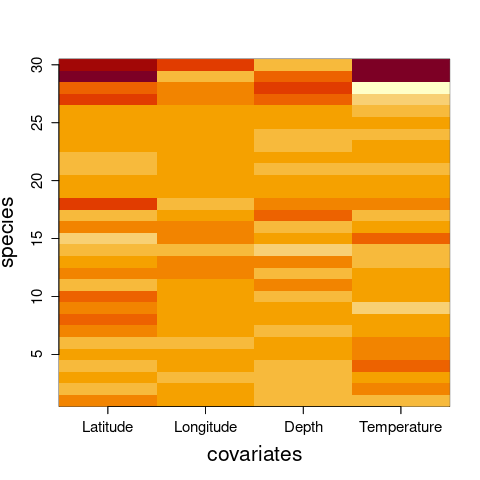
\includegraphics[width=.25\textwidth, trim=0 10 20 10, clip=]{\figbayes/FigUVSQ-BarentsFish-coeffAll-woIntercept-specOrderTRUE} & 
    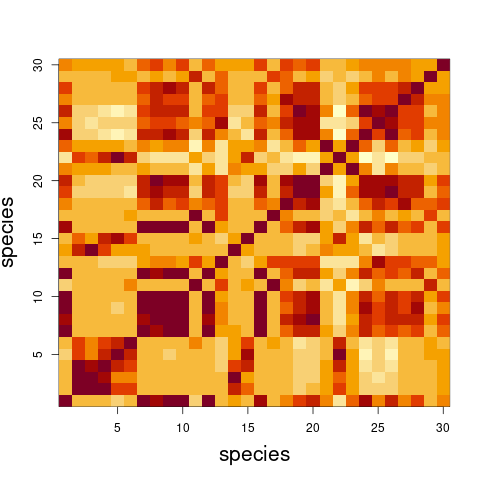
\includegraphics[width=.25\textwidth, trim=0 10 20 10, clip=]{\figbayes/FigUVSQ-BarentsFish-corrPred-specOrderTRUE} & 
    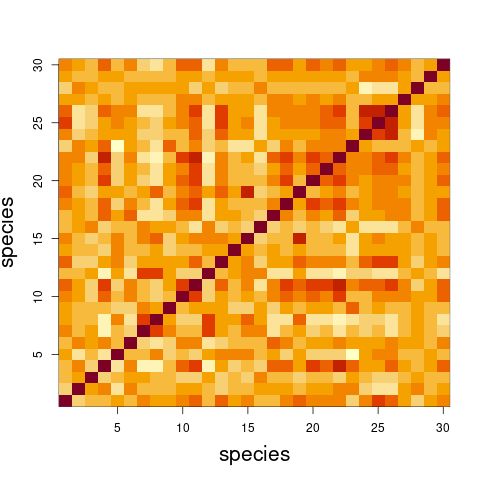
\includegraphics[width=.25\textwidth, trim=0 10 20 10, clip=]{\figbayes/FigUVSQ-BarentsFish-corrAll-specOrderTRUE}
  \end{tabular}
  $$
}

%====================================================================
%====================================================================
\subsection{From EM to Variational EM}
% \frame{\frametitle{Outline} \tableofcontents[currentsubsection]}
%====================================================================
\frame{\frametitle{Maximum likelihood with latent variables}

  \paragraph{Latent variable model.} Three ingredients:
  \begin{enumerate}
    \item $\emphase{\theta} =$ set of parameters:
    \begin{align*}
      \text{PLN:} \quad \theta & = (B, \Sigma) &
      \text{SBM:} \quad \theta & = (\pi, \alpha, \beta)
    \end{align*}
    \item $\emphase{Z} =$ set of latent variables:
    \begin{align*}
      Z & \sim p_\theta(Z) &
      (\text{PLN:\; multivariate normal, SBM:\; multinomial})
    \end{align*}
    \item $\emphase{Y} =$ set of observed variables:
    \begin{align*}
      Y & \sim p_\theta(Y \mid Z) &
      (\text{PLN \& SBM:\; Poisson})
    \end{align*}
  \end{enumerate}

  \bigskip \bigskip \pause
  \paragraph{Maximum likelihood inference.} Estimate $\theta$ with
  $$
  \widehat{\theta}
  = \argmax_\theta \; \log p_\theta(Y) 
  = \argmax_\theta \; \log \underset{\text{\normalsize Most often intractable}}{\underbrace{\int p_\theta(Y \mid z) p_\theta(z) \d z}} 
  $$

}

%====================================================================
\frame{\frametitle{EM algorithm}

  \paragraph{Expectation-Maximisation algorithm \refer{DLR77}.} $\theta^{(h)} =$ current value of the estimate,
  \begin{itemize}
    \item \emphase{E} step: Evaluate
    $$
    Q(\theta \mid \theta^{(h)}) := \Esp_{\theta^{(h)}}\left[\emphase{\log p_\theta(Y, Z)} \mid Y\right]
    $$
    \item \emphase{M} step: Update
    $$
    \theta^{(h+1)} = \argmax_\theta Q(\theta \mid \theta^{(h)})
    $$
  \end{itemize}
  $\to$ The log-likelihood increases at each step: $\log p_{\theta^{(h+1)}}(Y) \geq \log p_{\theta^{(h)}}(Y)$ .
  
  \bigskip \bigskip \pause
  \paragraph{Critical step = E step:} Requires to determine the conditional distribution
  $$
  p_\theta(Z \mid Y),
  $$
  or at least some of its moments.

  
  \bigskip \bigskip \pause
  \paragraph{Problem.} 
  For many models (including PLN and SBM), the E step is intractable 
}

%====================================================================
\frame{\frametitle{Variational EM (VEM) algorithm}

  \bigskip
  \paragraph{Principle \refer{WaJ08,BKM17}.} Replace the E step with an approximation step, i.e. \\ ~
  \begin{itemize}
    \setlength{\itemsep}{1\baselineskip}
    \item \pause Choose a class $\Qcal$ of approximate (parametric) distributions
    \item \pause Choose divergence measure $D[q \| p]$ (e.g. $KL[q \| p]$)
    \item \pause \emphase{VE} step : (approximation)
    $$
    q^{(h+1)} = \argmin_{q \in \emphase{\Qcal}} \emphase{D}\left[q(Z) \| p_{\theta^{(h)}}(Z \mid Y)\right]
    $$
    \item \pause \emphase{M} step : (update)
    $$
    \theta^{(h+1)} = \argmax_\theta \Esp_{\emphase{q^{(h+1)}}}\left[\log p_\theta(Y, Z)\right]
    $$
  \end{itemize}
  \pause
  \bigskip
  $\to$ If $D = KL$, a lower bound of $\log p_\theta(Y)$ ('ELBO') increases at each step
}
  
%====================================================================
\frame{\frametitle{Variational estimates}

  \bigskip 
  \textcolor{gray}{\paragraph{Remark:} A Bayesian version of it exists (Variational Bayes EM = VBEM).}

  \bigskip \bigskip \pause
  \paragraph{Pros:} Reasonably easy to implement, fast, empirically accurate
  
  \bigskip \bigskip \pause
  \paragraph{Cons:} Few theoretical guaranties \refer{CDP12,BCC13,MaM15}, does not enjoy the general properties of maximum likelihood (consistency, asymptotic normality, etc.) \\
  \medskip 
  $\to$ No measure of uncertainty (\emphase{no test, no confidence interval}) 
  
  \bigskip \bigskip \pause
  \paragraph{Question:} 
  Can we build upon variational inference to achieve 'genuine' statistical inference?

}

%====================================================================
%====================================================================
\subsection{Species abundances: Poisson log-normal model}
% \frame{\frametitle{Outline} \tableofcontents[currentsubsection]}
%====================================================================
\frame{\frametitle{Example 1: Variational EM (VEM) for the Poisson log-normal model}

  \paragraph{Model.} 
  $n$ sites, $p$ species
  \begin{align*}
    & \text{in each site $i = 1 \dots n$:} & 
    \emphase{Z_i} & \sim \Ncal_p(0, \emphase{\Sigma}) &
    & (\text{latent vector}) \\
    & \text{for each species $j = 1 \dots p$:} &
    Y_{ij} \mid Z_{ij} & \sim \Pcal(\exp(x_i^\top \emphase{\beta_j} + Z_{ij})) &
    & (\text{observed abundances})
  \end{align*} 
  
  \bigskip \pause
  \paragraph{No EM.} 
  The $Z_i$'s are marginally Gaussian, but not Gaussian conditionally on the $Y_{ij}$'s \\
  (no close form for $p(Z \mid Y)$, even in one dimension)
  
  \bigskip \bigskip \pause
  \paragraph{Variational EM.} Gaussian approximation \refer{CMR18a}
  $$
  q(Z) = \prod_{i=1}^n \Ncal(Z_i; m_i, S_i)
  $$
  \begin{itemize}
  \item Parameter estimate $\widehat{\theta} = (\widehat{\Sigma}, \widehat{\beta})$, 
  \item Approximate conditional distribution $Z_i \mid Y_i \approx \Ncal(\widetilde{m}_i, \widetilde{S}_i)$, 
  \item Lower bound $ELBO(\widehat{\theta}, \widetilde{m}, \widetilde{S})$ (R package \url{PLNmodels})
  \end{itemize}
  
}

%====================================================================
\frame{\frametitle{Toward genuine maximum likelihood inference \refer{StR24}}

  \pause
  \paragraph{Monte Carlo EM.} \refer{CeD85} When $p(Z \mid Y)$ intractable:
  \begin{itemize}
    \item Monte Carlo E step: Sample $(Z^m)_{m = 1 \dots M} \overset{iid}{\sim} p_{\theta^{(h)}}(Z \mid Y)$, then estimate
    $$
    \widehat{Q}(\theta \mid \theta^{(h)}) := \frac1{M} \sum_{m=1}^M \log p_\theta(Y, Z^m)
    $$
    \item M step: Update
    $$
    \theta^{(h+1)} = \argmax_\theta \widehat{Q}(\theta \mid \theta^{(h)}) 
    $$
  \end{itemize}

  \bigskip \bigskip \pause
  \paragraph{Importance sampling. }
  How to sample from $p_{\theta^{(h)}}(Z \mid Y)$?
  \begin{itemize}
   \item Sample $(Z^m)_{m = 1 \dots M} \overset{iid}{\sim} q^{(h)}(Z)$, $q^{(h)} =$ proposal,
   \item Compute the non-normalized weights $\rho_m^{(h)} = p_{\theta^{(h)}}(Y, Z^m) \left/ q^{(h)}(Z^m)\right.$,
   \item \pause Estimate
    $$
    \widehat{Q}(\theta \mid \theta^{(h)}) := \sum_{m=1}^M \rho_m^{(h)} \log p_\theta(Y, Z^m) \; \left/ \; \sum_{m=1}^M \rho_m^{(h)} \right.,
    $$
  \end{itemize}

}

%====================================================================
\frame{\frametitle{Composite likelihood}

  \bigskip
  \paragraph{Importance sampling has a poor efficiency\footnote{Measured in terms of ESS $\simeq$ variance of the weights}} in 'large' dimension (say $p \geq 10, 15$) \\
  \medskip 
  $\to$ Need to reduce the sampling dimension

  \bigskip \bigskip \pause
  \paragraph{Composite likelihood.} 
  \begin{itemize}
    \item Build $B$ overlapping blocks $\Ccal_1, \dots \Ccal_B$, each containing $k$ species, 
    \item Define the composite log-likelihood as
    $$
    \cl_\theta(Y) = \sum_{b=1}^B \log p_\theta(Y^b), 
    \qquad
    \text{where} \quad 
    Y^b = [Y_{ij}]_{i = 1, \dots n, j \in \Ccal_b},
    $$
    \item \pause Then, the maximum composite likelihood estimator \refer{VRF11}
    $$
    \widehat{\theta}_{CL} = \argmax_\theta \cl_\theta(Y) 
    $$
    is consistent, asymptotically Gaussian with asymptotic variance given by
    \begin{align*}
      J(\theta) & = \Var_\theta[\nabla_\theta \cl_\theta(Y)], 
      \qquad \qquad 
      H(\theta) = - \Esp_\theta[\nabla^2_\theta \cl_\theta(Y)], \\
      \Var_\infty(\widehat{\theta}_{CL}) & = H^{-1}(\theta) J(\theta) H^{-1}(\theta).
    \end{align*} 
  \end{itemize}

}

%====================================================================
\frame{\frametitle{Proposed composite likelihood algorithm}

  \paragraph{Dealing with latent variables.}
  \begin{itemize}
    \item The latent variables $Z$ can be split in the same way as the observed abundances $Y$:
    $$
    Z^b = [Z_{ij}]_{i = 1, \dots n, j \in \Ccal_b},
    $$
    \item The EM algorithm can be extended to composite log-likelihood \\
    \textcolor{gray}{(Proof: apply the EM decomposition within each block)}
  \end{itemize}

  \bigskip \bigskip \pause
  \paragraph{Proposal for importance sampling.}
  \begin{itemize}
    \item Start with $q_b^{(1)}(Z^b) = \qt_{VEM}(Z^b)$
    \item Then update $q_b^{(h+1)}(Z^b)$ with the estimated mean and variance of $p_{\theta^{(h)}}(Z^b \mid Y^b)$.
  \end{itemize}

  \bigskip \bigskip \pause
  \paragraph{Building the blocks.} To guaranty the same precision for all estimates, one would ideally want that
  \begin{itemize}
    \item[$\beta_j$:] Each species $j$ belongs to the same number of blocks $\Ccal_1, \dots \Ccal_B$
    \item[$\sigma_{jj'}$:] Each pair of species $(j, j')$ appears in the same number of blocks 
    \item Same problem as the construction of a incomplete balanced block design\footnote{Not always possible: need to have $p \mid Bk$ and $p(p-1) \mid Bk(k-1)$}
  \end{itemize}

}

%====================================================================
\frame{\frametitle{Simulation study}

  \paragraph{Main aim.} Assess normality 
  \begin{itemize}
    \item Test statistic $(\widehat{\theta} -\theta^*) \left/ \sqrt{\widehat{\Var}_\infty(\widehat{\theta})} \right.$ for the regression coefficients
    \item Criterion = $p$-value of the Kolmogorov-Smirnov test for normality
  \end{itemize}
  
  \bigskip \bigskip \pause
  \paragraph{Results.} $100$ sites, $3$ covariates, $100$ simulations
  \newcommand{\lagSim}{50} \newcommand{\nISsim}{200} \newcommand{\nIterSim}{1000}
  \newcommand{\simulParms}{-nIter\nIterSim-lag\lagSim-nIS\nISsim}
  $$
  \begin{tabular}{cccc}
    7 species & 10 species & 20 species & 50 species \\
    \includegraphics[width=.2\textwidth, trim=10 10 25 25, clip=]{\figStR/PvalKS-score-n100-d3-p7-parm1\simulParms} & 
    \includegraphics[width=.2\textwidth, trim=10 10 25 25, clip=]{\figStR/PvalKS-score-n100-d3-p10-parm1\simulParms} & 
    \includegraphics[width=.2\textwidth, trim=10 10 25 25, clip=]{\figStR/PvalKS-score-n100-d3-p20-parm1\simulParms} &
    \includegraphics[width=.2\textwidth, trim=10 10 25 25, clip=]{\figStR/PvalKS-score-n100-d3-p50-parm1\simulParms}  
  \end{tabular}
  $$
  FL = full likelihood, CL$k$ = composite likelihood$(k = \textcolor{gray}{2}, 3, \textcolor{gray}{5}, 7)$, \\
  \medskip
  \textcolor{gray}{VEM = pseudo Fisher information based on the ELBO},  \\
  JK = jackknife variance estimate of $\Var(\widehat{\theta}_{VEM})$

}

%====================================================================
\frame{\frametitle{Fish species in the Barents sea}

  \newcommand{\nIterEx}{10000} \newcommand{\lagEx}{50} \newcommand{\nISex}{200}
  \newcommand{\exampleParms}{-nIter\nIterEx-lag\lagEx-nIS\nISex}
  \newcommand{\nIterSel}{\nIterEx} \newcommand{\lagSel}{20} \newcommand{\nISsel}{\nISex}
  \newcommand{\selectParms}{-nIS\nISsel-nIter\nIterSel-lag\lagSel}
  
  \bigskip
  \paragraph{Comparison of the estimates.}
  $$
  \begin{tabular}{ccc}
    $\widehat{B}$ & $\widehat{\Sigma}$ & ESS (CL5) \\
    \includegraphics[width=.25\textwidth, trim=10 10 25 50, clip=]{\figStR/Barents\exampleParms-compBeta-cem5-all} & 
    \includegraphics[width=.25\textwidth, trim=10 10 25 50, clip=]{\figStR/Barents\exampleParms-compSigma-cem5-all} & 
    \includegraphics[width=.25\textwidth, trim=10 10 25 50, clip=]{\figStR/Barents\exampleParms-ESS-cem5}     
  \end{tabular}
  $$

  \pause
  \paragraph{Significance.} Test statistics $\widehat{\theta} \left/ \sqrt{\widehat{\Var}_\infty(\widehat{\theta})} \right.$
  $$
  \begin{tabular}{ccc}
    $\widehat{B}$ & $\widehat{\Sigma}$ & $\text{cor}(\widehat{\Sigma})$ \\
    \includegraphics[width=.25\textwidth, trim=10 10 25 25, clip=]{\figStR/Barents\exampleParms-betaSignif-cem5} & 
    \includegraphics[width=.25\textwidth, trim=10 10 25 25, clip=]{\figStR/Barents\exampleParms-sigmaSignif-cem5} &
    \includegraphics[width=.25\textwidth, trim=10 10 25 25, clip=]{\figStR/Barents\exampleParms-corSigmaSignif-cem5}
  \end{tabular}  
  $$
}


